\section*{Anhang~A: Persona-Skizze}\label{sec:anhang_a}

\begin{table}[H]
\caption{Persona-Skizze: Mara K., nachhaltigkeitsorientierte Hobbyköchin}\label{tab:persona}
{\footnotesize
\begin{tabularx}{\textwidth}{@{}l X@{}}
\toprule
\textbf{Merkmal} & \textbf{Beschreibung} \\
\midrule
& 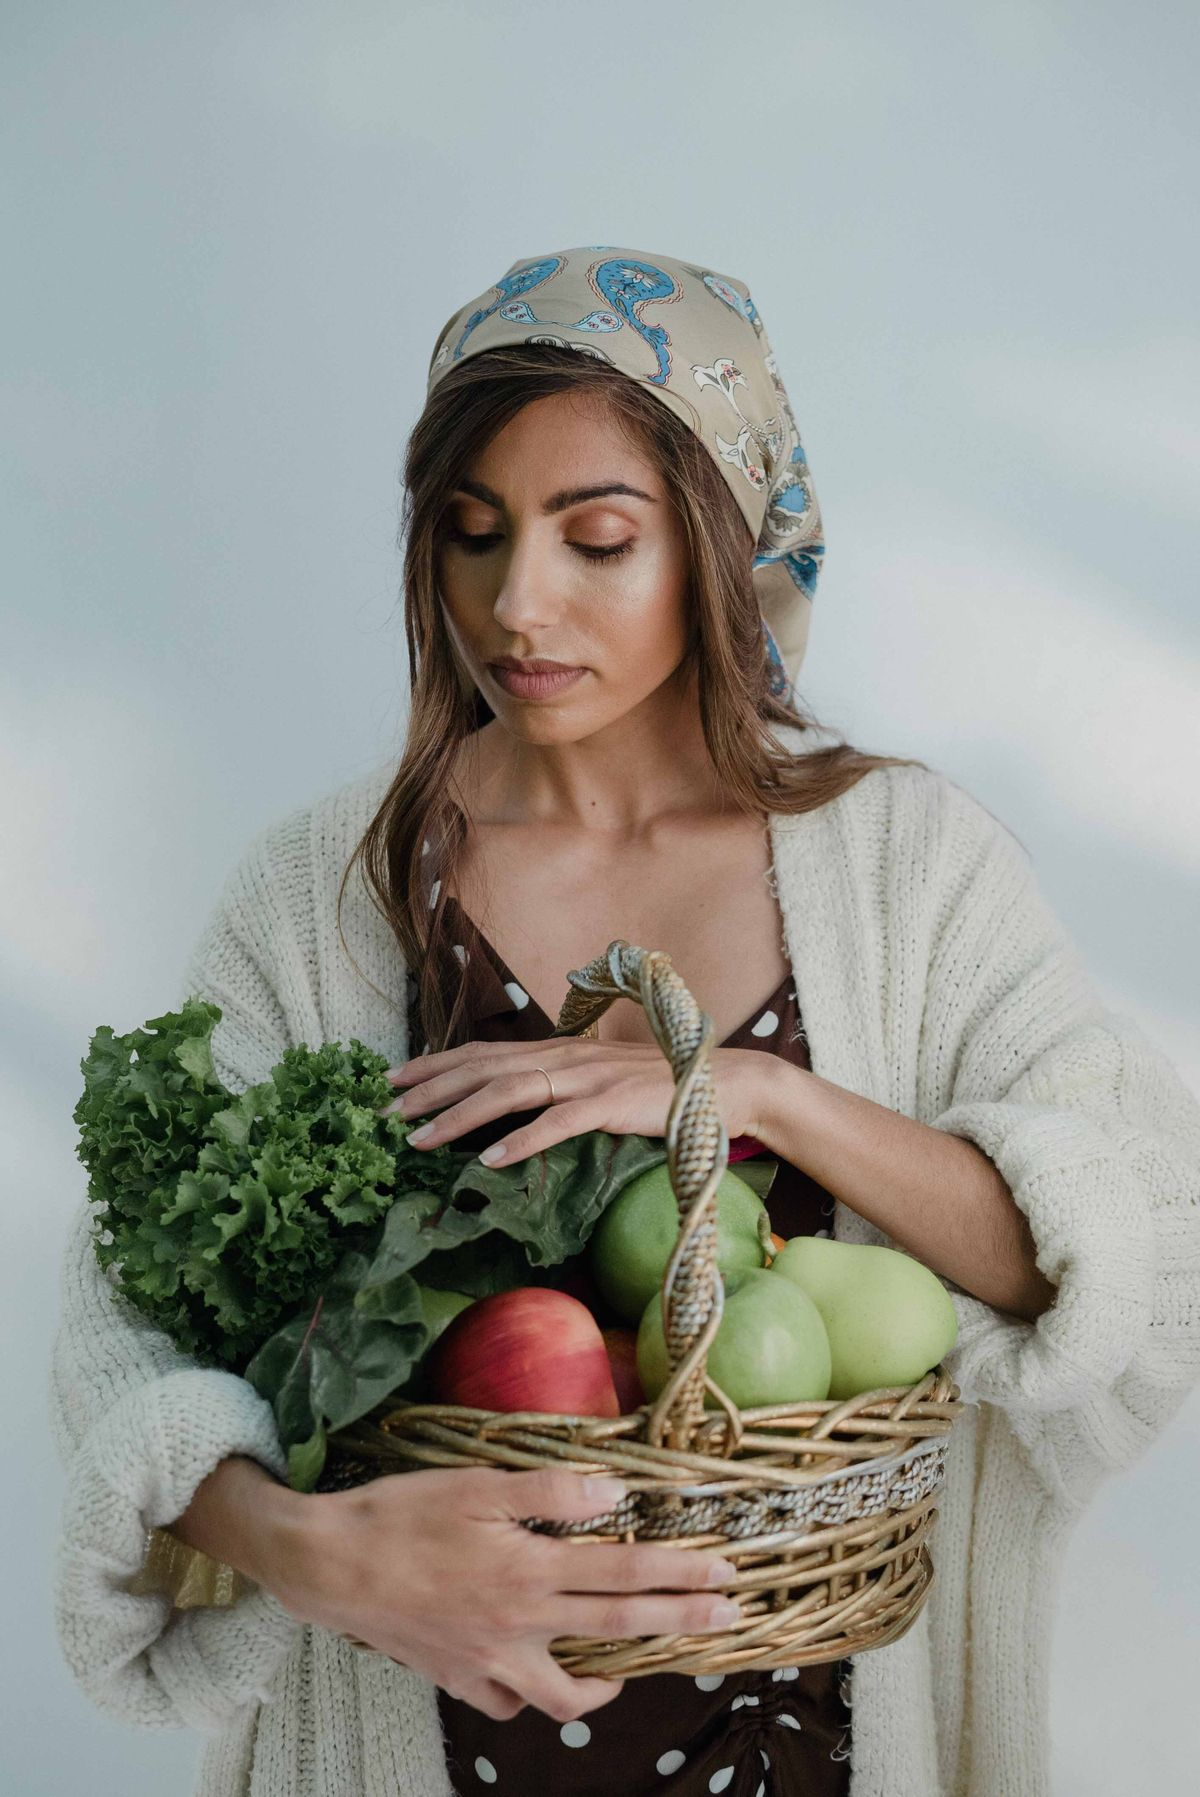
\includegraphics[width=4.5cm]{images/durchfuehrung/persona_mara.jpg} \\
Name (fiktiv) & Mara K. \\
Alter & 29 Jahre \\
Lebenssituation & Vollzeit berufstätig, kocht vier- bis fünfmal pro Woche selbst \\
Motivation & Möchte vorhandene Lebensmittel konsequent verwerten und hat sich zunehmend mit Nachhaltigkeit im Alltag beschäftigt \\
Painpoint & Findet online häufig Rezepte, die zusätzliche Zutaten verlangen, statt vorhandene Reste zu nutzen; hat wenig Zeit für aufwendige Planung \\
Zero-Waste-Bezug & Kauft gezielt kleine Mengen ein, ärgert sich aber, wenn Reste ungenutzt bleiben \\
Typische Haltung & Möchte nicht extra einkaufen müssen, nur weil ein Rezept eine Zutat verlangt, die zu Hause ohnehin fehlt \\
\bottomrule
\end{tabularx}
}
\quelle{Eigene Darstellung. Portraitfoto: \citeauthor{pexelsHasanbekavaBasket}, \citeyear{pexelsHasanbekavaBasket}. Pexels-Lizenz.}
\end{table}

\section*{Anhang~B: Style Tile Resteria}\label{sec:anhang_b}

\begin{figure}[H]
\caption{Style Tile Resteria: Farbwelt, Typografie und wiederkehrende Bedienelemente}\label{fig:styletile}
\centering
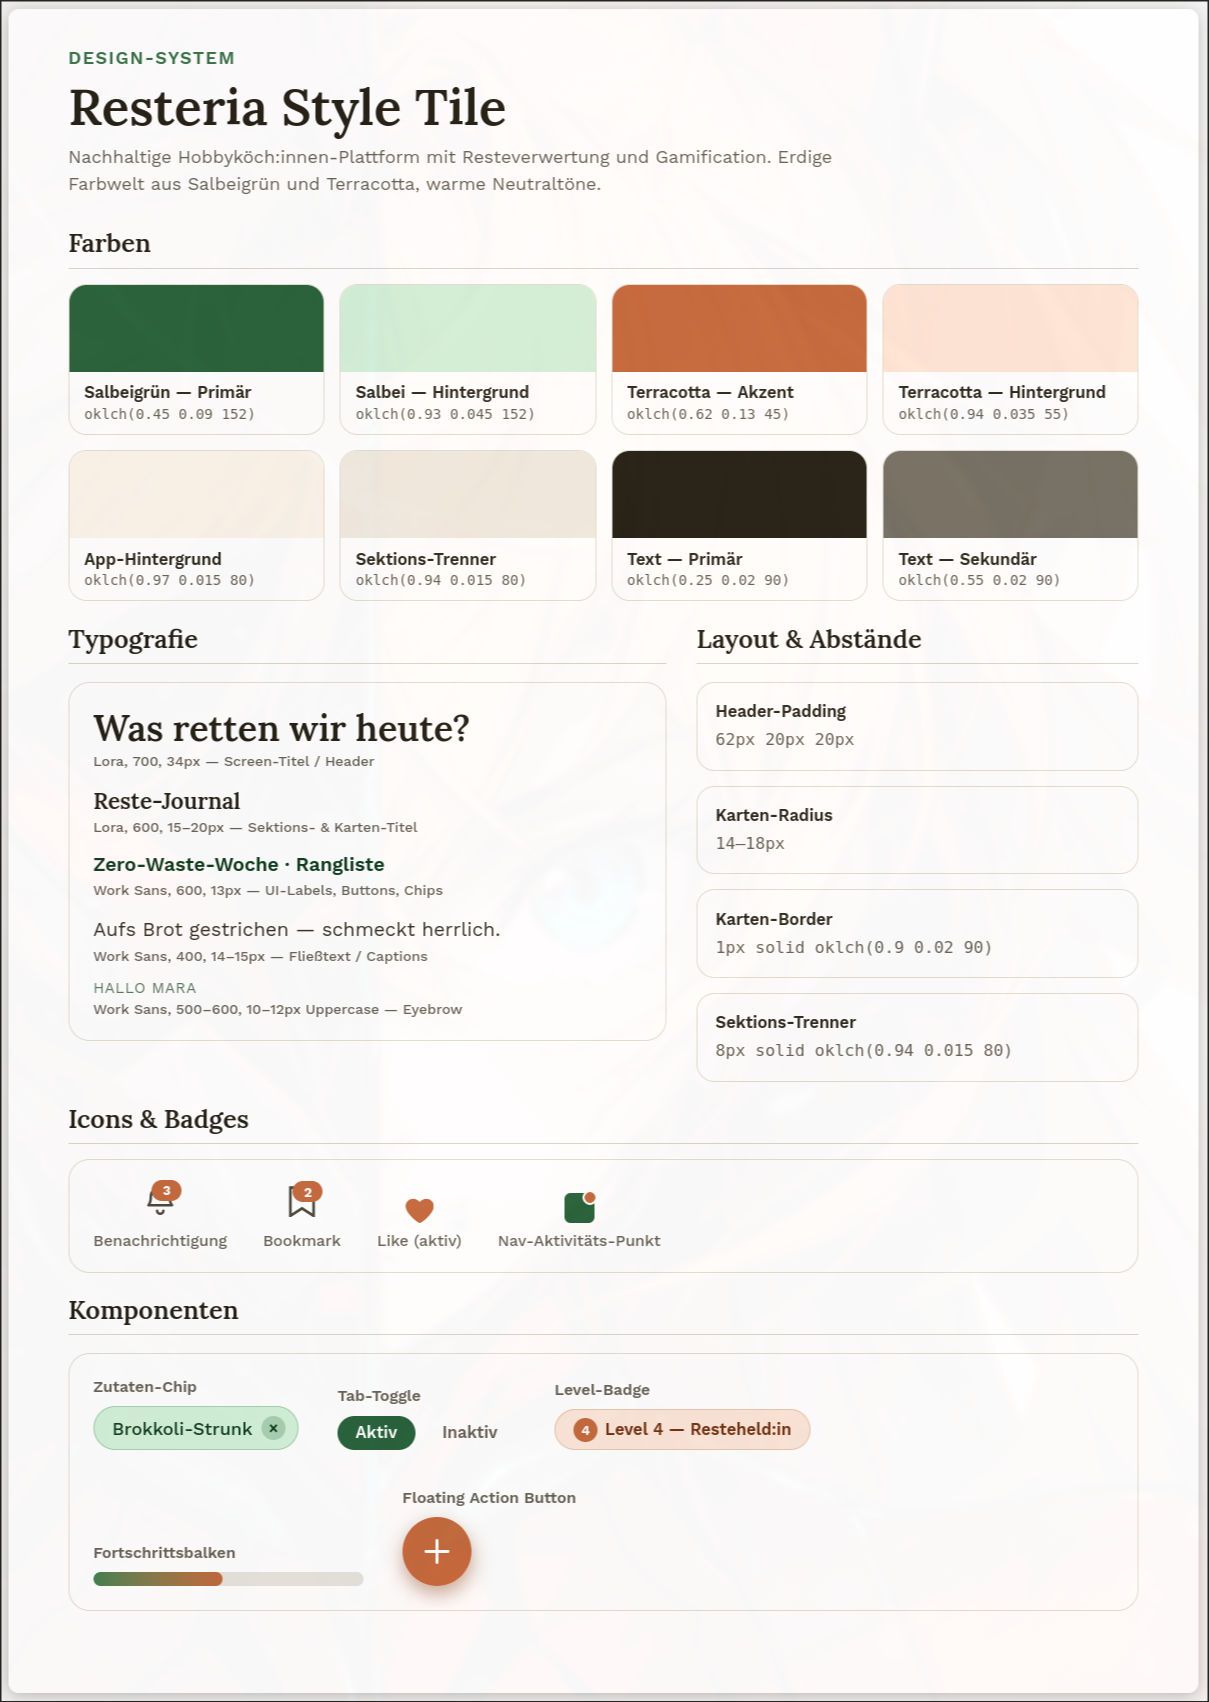
\includegraphics[height=0.85\textheight, keepaspectratio]{images/durchfuehrung/resteria_styletile.png}
\quelle{Erstellt mit dem Prompt \enquote{Erstelle einen Style Tile für das Projekt auf einer neuen Seite. Formatiere ihn als kompakter One-Pager im A4 Seitenformat} durch Anthropic, 2026 (Claude Design, Modell Claude Sonnet 5).}
\end{figure}

\section*{Anhang~C: UI/UX-Mockups Resteria}\label{sec:anhang_c}

\begin{figure}[H]
\caption{UI/UX-Mockup Resteria: Startseite mit Reste-Eingabe und Rezeptvorschlag}\label{fig:mockup_start}
\centering
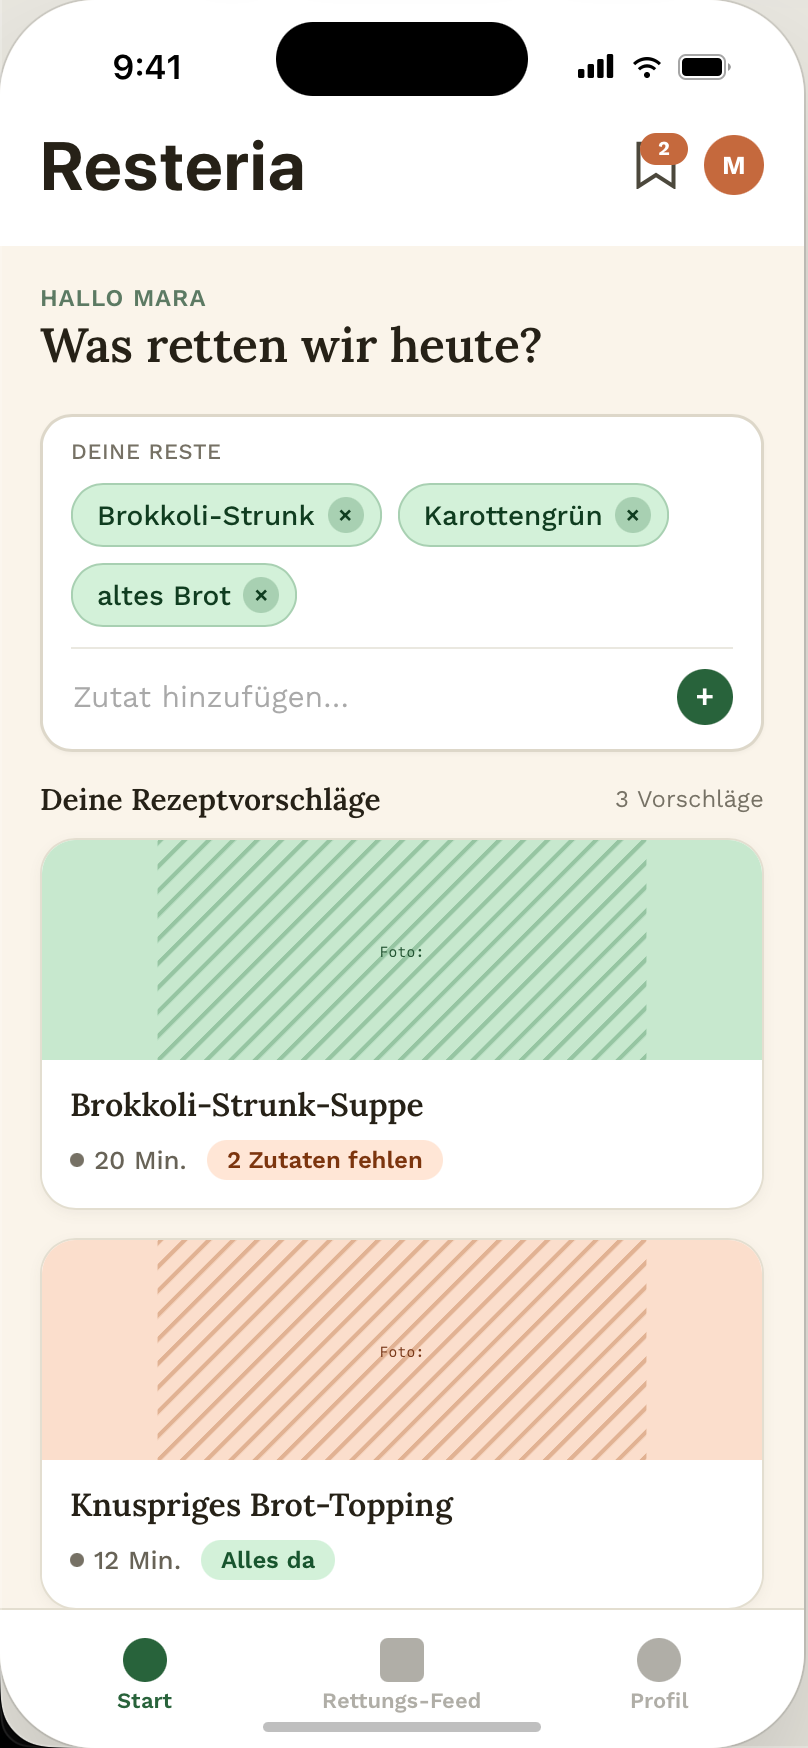
\includegraphics[height=0.55\textheight, keepaspectratio]{images/durchfuehrung/resteria_startseite.png}
\quelle{Erstellt mit dem Prompt \enquote{Mobiler App-Screen für Resteria, eine Social-Media-Plattform für nachhaltigkeitsorientierte Hobbyköche: Startseite mit Reste-Eingabefeld (Zutaten als Chip-Tags, z.\,B. Brokkoli-Strunk, Karottengrün, altes Brot) darunter Rezeptvorschläge als Karten mit Zubereitungszeit und fehlenden Zutaten. Verwende einen warmen, erdigen Look in Grün- und Terracotta-Tönen, keine Stock-Photo-Ästhetik}, in weiteren Iterationsschritten verfeinert, durch Anthropic, 2026 (Claude Design, Modell Claude Sonnet 5). Abbildung nachträglich manuell bearbeitet.}
\end{figure}

\begin{figure}[H]
\caption{UI/UX-Mockup Resteria: Startseite mit ausgeklappten gespeicherten Rezepten}\label{fig:mockup_start_bookmarks}
\centering
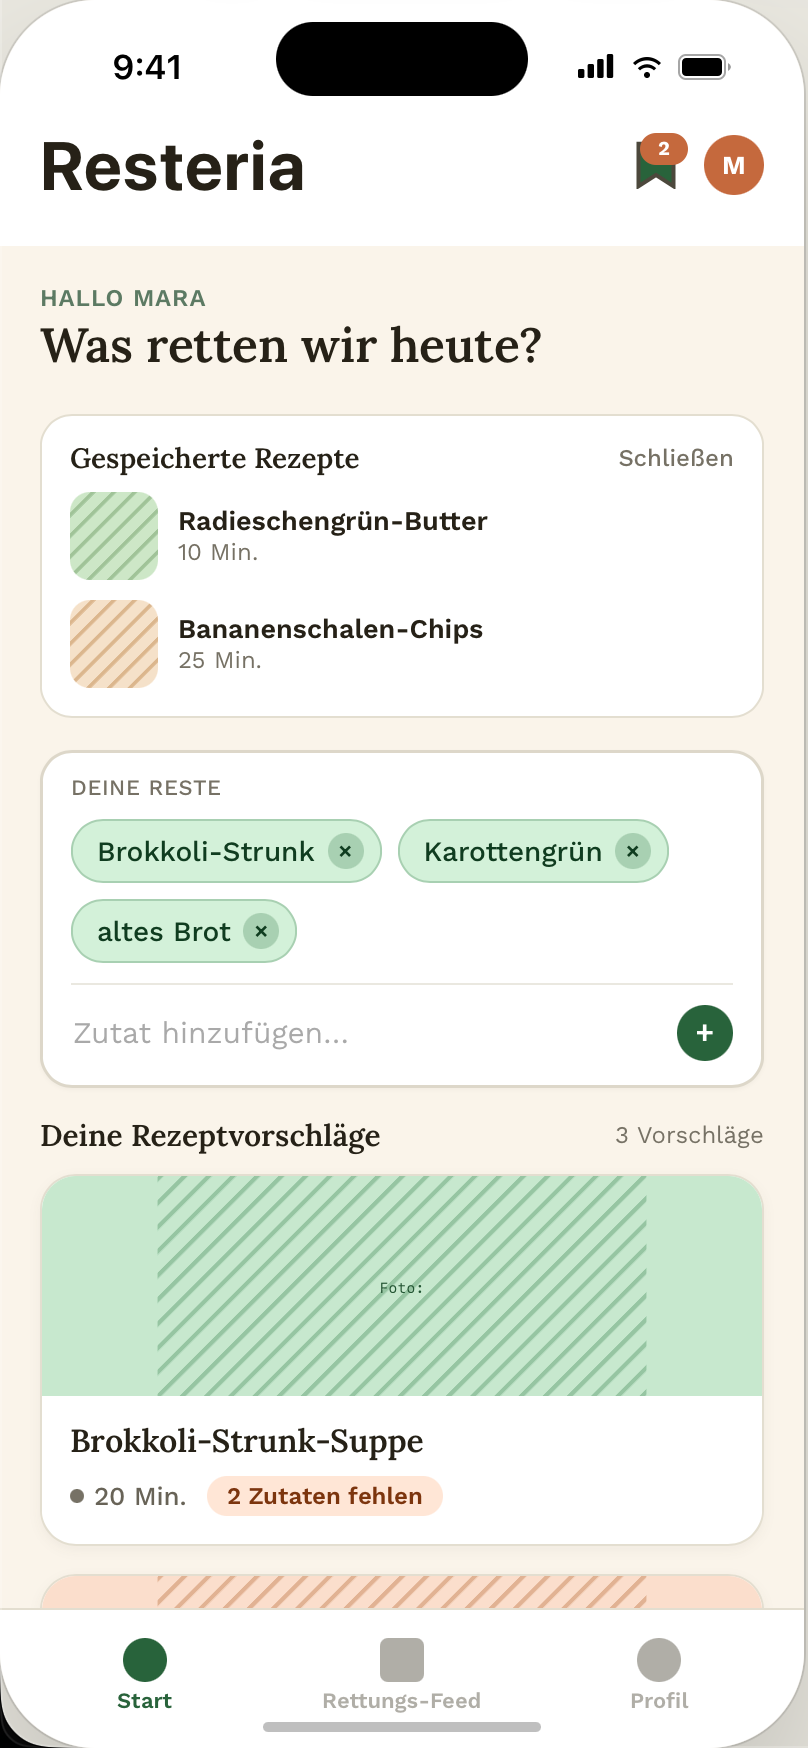
\includegraphics[height=0.55\textheight, keepaspectratio]{images/durchfuehrung/resteria_startseite_bookmarks.png}
\quelle{Erstellt mit dem Prompt \enquote{Ergänze ein über das Lesezeichen-Icon ausgeklappten Bereich \enquote{Gespeicherte Rezepte}, der zuvor per Lesezeichen markierte Rezeptvorschläge auflistet.}, in weiteren Iterationsschritten verfeinert, durch Anthropic, 2026 (Claude Design, Modell Claude Sonnet 5). Abbildung nachträglich manuell bearbeitet.}
\end{figure}

\begin{figure}[H]
\caption{UI/UX-Mockup Resteria: Rettungs-Feed}\label{fig:mockup_feed}
\centering
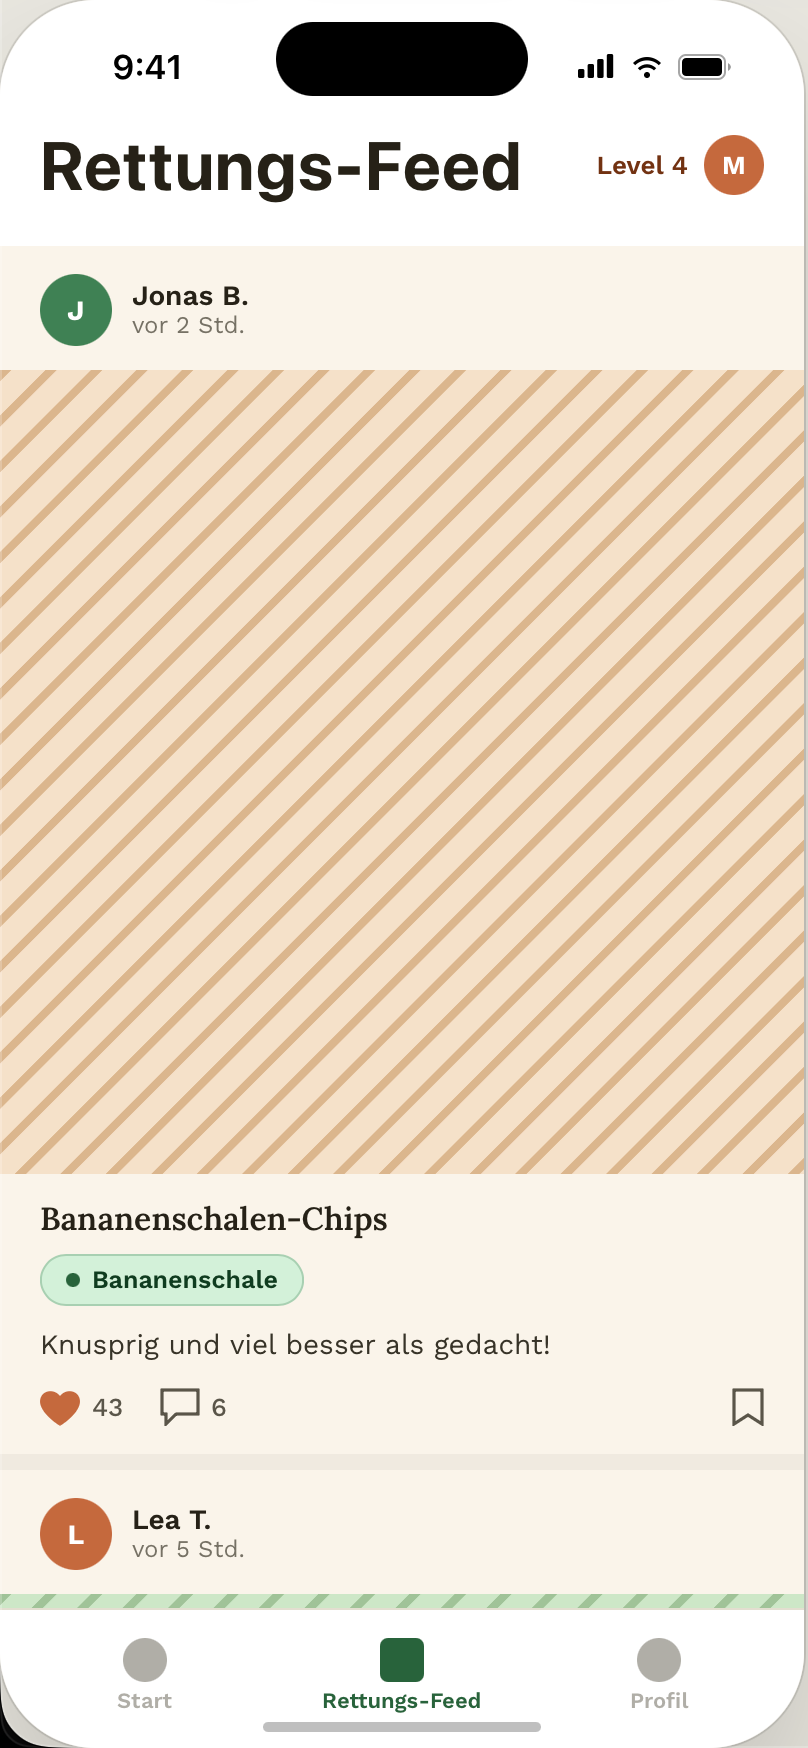
\includegraphics[height=0.55\textheight, keepaspectratio]{images/durchfuehrung/resteria_rettungsfeed.png}
\quelle{Erstellt mit dem Prompt \enquote{Rettungs-Feed im Social-Media-Stil mit Beiträgen, mit je ein Foto, Nutzernamen, Tags mit geretteten Zutaten sowie Like- und Kommentar-Icons. Warmer, erdiger Look in Grün- und Terracotta-Tönen, keine Stock-Photo-Ästhetik}, ergänzt um die Folge-Prompts \enquote{Ergänze am Rettungs-Feed-Screen einen schwebenden Terracotta-Plus-Button unten rechts zum Beitrag-Erstellen sowie ein schmales Challenge-Banner oben für die \enquote{Zero-Waste-Woche}-Rangliste}, in weiteren Iterationsschritten verfeinert, durch Anthropic, 2026 (Claude Design, Modell Claude Sonnet 5). Abbildung nachträglich manuell bearbeitet.}
\end{figure}

\begin{figure}[H]
\caption{UI/UX-Mockup Resteria: Profil mit Rettungspunkten und Reste-Level}\label{fig:mockup_profil}
\centering
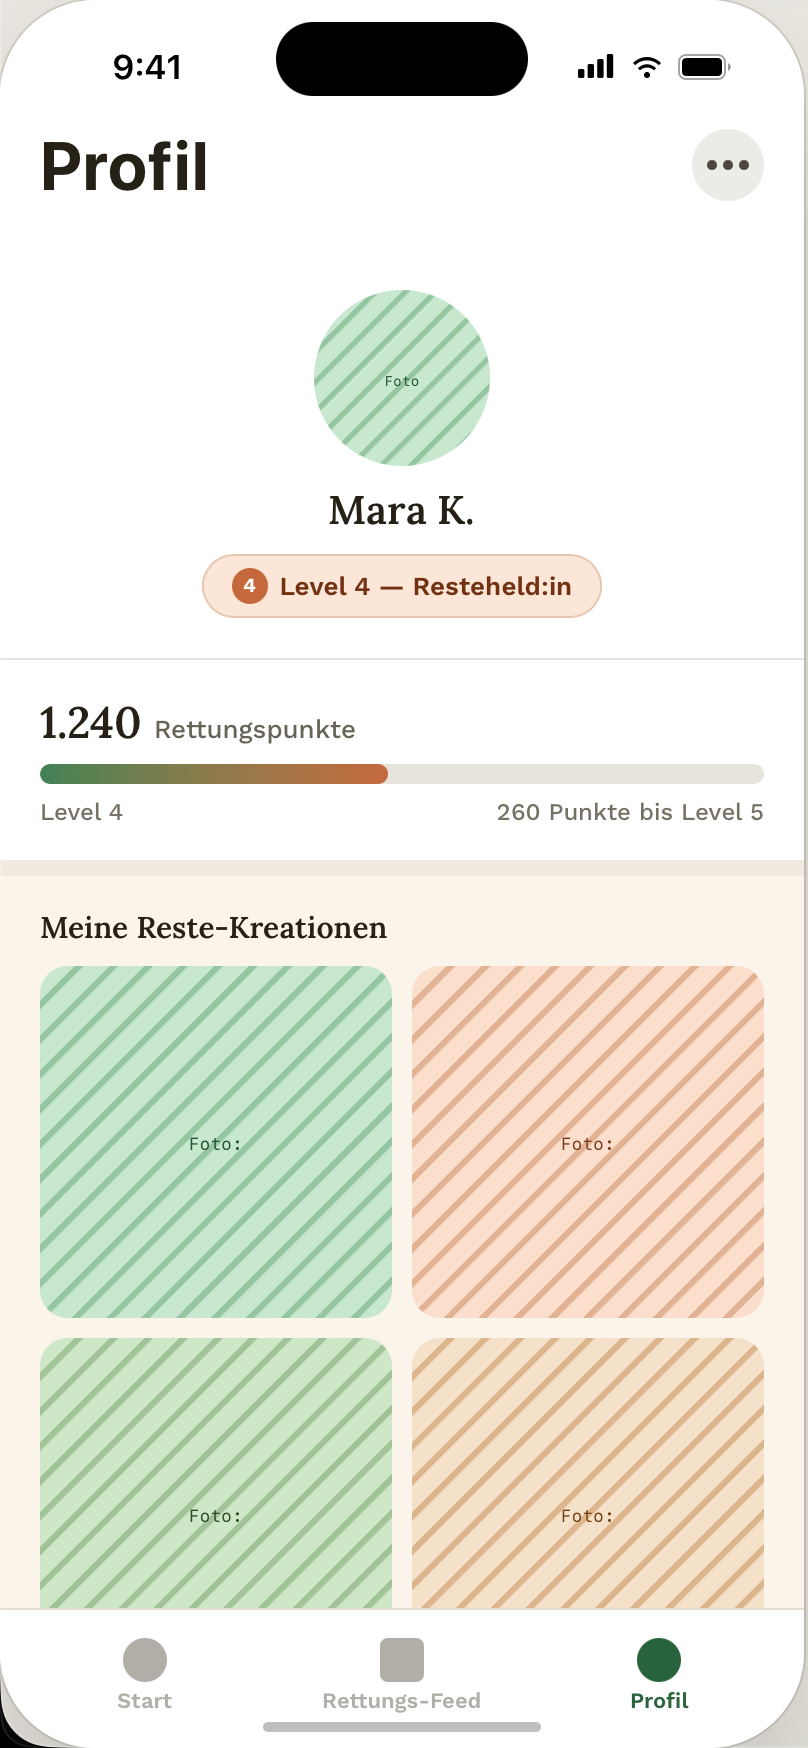
\includegraphics[height=0.55\textheight, keepaspectratio]{images/durchfuehrung/resteria_profil.png}
\quelle{Erstellt mit dem Prompt \enquote{Profilbereich mit Profilbild Platzhalter, Name und Reste-Level-Badge (z.\,B. \enquote{Level 4 - Resteheld}), Rettungspunkte-Fortschrittsbalken und einem Raster eigener geposteter Reste-Kreationen. Warmer, erdiger Look in Grün- und Terracotta-Tönen, keine Stock-Photo-Ästhetik}, ergänzt um die Folge-Prompts \enquote{Ergänze unterhalb des Rettungspunkte-Fortschrittsbalkens eine zweite, kleinere Kennzahl mit einer konkreten Mengenangabe, z.\,B. \enquote{12,4 kg Lebensmittel gerettet}}, in weiteren Iterationsschritten verfeinert, durch Anthropic, 2026 (Claude Design, Modell Claude Sonnet 5). Abbildung nachträglich manuell bearbeitet.}
\end{figure}
